\documentclass[aspectratio=169,10pt,xcolor=table]{beamer}

\usepackage[T1]{fontenc}
\usepackage[utf8]{inputenc}
\usepackage{lmodern}
\usepackage{booktabs}
\usepackage{array}
\usepackage{listings}
\usepackage{tikz}
\usetikzlibrary{arrows.meta,positioning,calc}

% Colors follow the PS10 assignment slide: Dining Philosophers red,
% Cigarette Smokers blue.
\definecolor{dp}{RGB}{176,0,0}
\definecolor{cs}{RGB}{0,112,192}
\definecolor{ok}{RGB}{0,128,64}
\definecolor{codegray}{gray}{0.95}

\hypersetup{colorlinks=true, linkcolor=cs, urlcolor=cs}

\setbeamercolor{frametitle}{fg=black}
\setbeamercolor{structure}{fg=cs}
\setbeamercolor{itemize item}{fg=cs}
\setbeamertemplate{navigation symbols}{}
\setbeamertemplate{frametitle}{%
    \vskip2.2ex
    {\usebeamerfont{frametitle}\insertframetitle\par}
    \vskip0.6ex
    {\color{cs}\hrule height 0.8pt}%
}
\setbeamertemplate{footline}{%
    \hfill\scriptsize\color{gray}%
    The Dining Philosophers vs.\ The Cigarette Smokers \quad
    \insertframenumber\hspace{2mm}\vspace{1.5mm}%
}
\setbeamertemplate{bibliography item}[text]
\setbeamerfont{frametitle}{size=\Large,series=\bfseries}

\lstset{
    language=Python,
    backgroundcolor=\color{codegray},
    basicstyle=\ttfamily\scriptsize,
    keywordstyle=\bfseries,
    commentstyle=\color{gray},
    frame=single,
    framerule=0pt,
    xleftmargin=2pt,
    aboveskip=2pt,
    belowskip=0pt,
    showstringspaces=false,
    columns=fullflexible
}

\newcommand{\code}[1]{\texttt{#1}}

\title{The Dining Philosophers vs.\ The Cigarette Smokers}
\subtitle{CPE333 Operating Systems -- Problem Session 10}
\author{
    Guntee Doungmanee (ID: 67070501003)\\
    Drarun Yookphan (ID: 67070501016)\\
    Rattathamnoon Buranapattana (ID: 67070501037)\\
    Supawit Marayat (ID: 67070501045)
}
\institute{King Mongkut's University of Technology Thonburi}
\date{}

\begin{document}

% ---------------------------------------------------------------- cover
\begin{frame}[plain]
    \titlepage
\end{frame}

% ---------------------------------------------------------------- 1
\begin{frame}{The Cigarette Smokers problem}
    \begin{columns}[T]
        \begin{column}{0.54\textwidth}
            \small
            \begin{itemize}
                \setlength\itemsep{2pt}
                \item Presented by Suhas Patil in 1971 \cite{patil,downey}.
                \item Four threads: one \textbf{agent}, three \textbf{smokers}.
                \item Ingredients: tobacco, paper, matches. Each smoker has an
                    infinite supply of \textbf{one} kind. The agent has an
                    infinite supply of all three \cite{downey}.
                \item The agent picks \textbf{two different} ingredients at
                    random and puts them on the table.
                \item The smoker with the \textbf{third} ingredient takes both,
                    makes and smokes a cigarette, then signals the agent. The
                    agent puts out two new ingredients.
            \end{itemize}
            \begin{block}{Premise \cite{downey}}
                \footnotesize The agent is an \textbf{operating system} that
                allocates resources. The smokers are \textbf{applications} that
                need them. Wake an application only when it can proceed, and
                always wake it when it can.
            \end{block}
        \end{column}
        \begin{column}{0.44\textwidth}
            \centering
            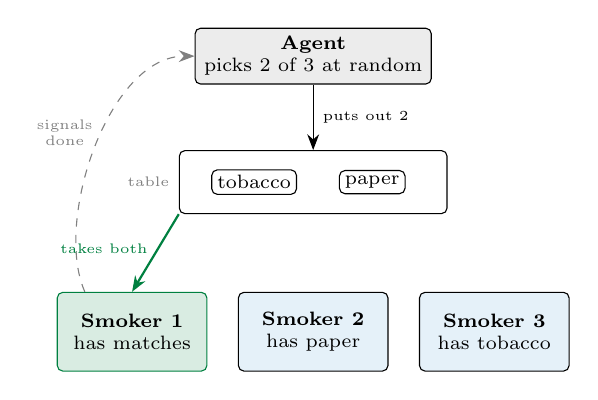
\begin{tikzpicture}[
                box/.style={draw, rounded corners=2pt, align=center, font=\scriptsize, inner sep=3pt},
                smoker/.style={box, fill=cs!10, minimum width=19mm, minimum height=10mm},
                item/.style={draw, fill=white, rounded corners=2pt, font=\scriptsize, inner sep=2pt},
                >={Stealth[length=2mm]}
            ]
                \node[box, fill=gray!15, minimum width=30mm] (agent) at (0,3.3)
                    {\textbf{Agent}\\picks 2 of 3 at random};
                \node[box, minimum width=34mm, minimum height=8mm, label={[font=\tiny,gray]left:table}] (table) at (0,1.7) {};
                \node[item] at (-0.75,1.7) {tobacco};
                \node[item] at (0.75,1.7) {paper};
                \node[smoker, fill=ok!15, draw=ok] (m) at (-2.3,-0.2) {\textbf{Smoker 1}\\has matches};
                \node[smoker] (p) at (0,-0.2) {\textbf{Smoker 2}\\has paper};
                \node[smoker] (t) at (2.3,-0.2) {\textbf{Smoker 3}\\has tobacco};
                \draw[->] (agent) -- node[right,font=\tiny]{puts out 2} (table);
                \draw[->, thick, ok] (table.south west) -- node[left,font=\tiny,pos=0.45]{takes both} (m.north);
                \draw[->, dashed, gray] ([xshift=-6mm]m.north) .. controls (-3.3,1.2) and (-2.6,3.3) .. (agent.west)
                    node[pos=0.55,left,font=\tiny,align=center]{signals\\done};
            \end{tikzpicture}
        \end{column}
    \end{columns}
\end{frame}

% ---------------------------------------------------------------- 2
\begin{frame}[fragile]{Why it is hard: the natural solution deadlocks}
    \begin{columns}[T]
        \begin{column}{0.55\textwidth}
            \small
            \textbf{Patil's restrictions} \cite{downey}
            \begin{enumerate}
                \setlength\itemsep{1pt}
                \item Do not change the agent code. The agent is the OS.
                \item No conditional statements and no array of semaphores.
            \end{enumerate}
            \footnotesize With both, Patil claimed semaphores cannot solve it.
            Parnas called restriction 2 artificial \cite{parnas,downey}.

            \vspace{5pt}
            \small\textbf{The natural solution} \cite{downey}\\
            \footnotesize Agent A runs \code{agentSem.wait()}, then
            \code{tobacco.signal()} and \code{paper.signal()}. Agents B and C
            are similar. The smokers:
            \vspace{2pt}

            \begin{minipage}[t]{0.47\textwidth}
\begin{lstlisting}
# Smoker with matches
tobacco.wait()
paper.wait()
agentSem.signal()
\end{lstlisting}
            \end{minipage}\hfill
            \begin{minipage}[t]{0.47\textwidth}
\begin{lstlisting}
# Smoker with tobacco
paper.wait()
match.wait()
agentSem.signal()
\end{lstlisting}
            \end{minipage}
        \end{column}
        \begin{column}{0.43\textwidth}
            \small
            \textbf{One bad schedule}
            \begin{enumerate}
                \setlength\itemsep{1pt}
                \item The agent puts out tobacco and paper.
                \item The matches smoker takes tobacco. The tobacco smoker takes paper.
                \item Each smoker now waits for something it cannot get.
            \end{enumerate}
            \vspace{2pt}
            \centering
            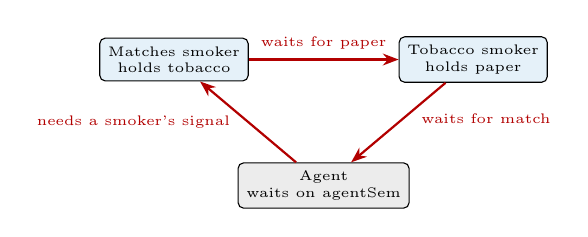
\begin{tikzpicture}[
                box/.style={draw, rounded corners=2pt, align=center, font=\tiny, inner sep=3pt, fill=cs!10},
                >={Stealth[length=2mm]}, lbl/.style={font=\tiny, red!70!black}
            ]
                \node[box] (m) at (-1.9,0) {Matches smoker\\holds tobacco};
                \node[box] (t) at (1.9,0) {Tobacco smoker\\holds paper};
                \node[box, fill=gray!15] (a) at (0,-1.6) {Agent\\waits on agentSem};
                \draw[->, thick, red!70!black] (m) -- node[above,lbl]{waits for paper} (t);
                \draw[->, thick, red!70!black] (t) -- node[right,lbl,pos=0.45,xshift=1mm]{waits for match} (a);
                \draw[->, thick, red!70!black] (a) -- node[left,lbl,pos=0.5,xshift=-1mm]{needs a smoker's signal} (m);
            \end{tikzpicture}

            \footnotesize The wait cycle includes the agent: \textbf{deadlock}
            \cite{downey}.
        \end{column}
    \end{columns}
\end{frame}

% ---------------------------------------------------------------- 3
\begin{frame}[fragile]{The solution: helper threads called pushers}
    \begin{columns}[T]
        \begin{column}{0.42\textwidth}
            \centering
            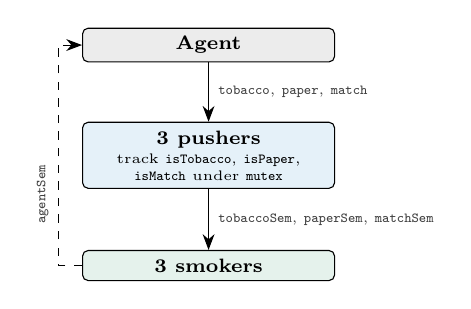
\begin{tikzpicture}[
                box/.style={draw, rounded corners=2pt, align=center, font=\scriptsize, inner sep=3pt, minimum width=32mm},
                >={Stealth[length=2mm]}, lbl/.style={font=\tiny, gray!50!black, align=left}
            ]
                \node[box, fill=gray!15] (a) at (0,2.6) {\textbf{Agent}};
                \node[box, fill=cs!10] (p) at (0,1.2) {\textbf{3 pushers}\\[-1pt]{\tiny track \code{isTobacco}, \code{isPaper},}\\[-2pt]{\tiny \code{isMatch} under \code{mutex}}};
                \node[box, fill=ok!10] (s) at (0,-0.2) {\textbf{3 smokers}};
                \draw[->] (a) -- node[right,lbl]{\code{tobacco}, \code{paper}, \code{match}} (p);
                \draw[->] (p) -- node[right,lbl]{\code{tobaccoSem}, \code{paperSem}, \code{matchSem}} (s);
                \draw[->, dashed] (s.west) -- ++(-0.3,0) |- node[left,lbl,pos=0.25,rotate=90,yshift=2mm]{\code{agentSem}} (a.west);
            \end{tikzpicture}

            \vspace{3pt}
            \footnotesize
            \begin{itemize}
                \setlength\itemsep{1pt}
                \item A smoker waits only on its own semaphore. The pushers signal
                    it only when \textbf{both} ingredients are on the table. No
                    smoker holds a partial set.
                \item Parnas indexes an array of semaphores with an integer. This
                    avoids conditionals \cite{parnas,downey}.
            \end{itemize}
        \end{column}
        \begin{column}{0.56\textwidth}
\begin{lstlisting}
# Pusher A: runs when the agent puts out tobacco
tobacco.wait()
mutex.wait()
if isPaper:                # paper is already there
    isPaper = False
    matchSem.signal()      # wake smoker with matches
elif isMatch:
    isMatch = False
    paperSem.signal()      # wake smoker with paper
else:
    isTobacco = True       # other item not here yet
mutex.signal()
\end{lstlisting}
\begin{lstlisting}
# Smoker with tobacco
tobaccoSem.wait()
makeCigarette()
agentSem.signal()
smoke()
\end{lstlisting}
            \vspace{2pt}
            \footnotesize Pushers B and C are similar. Code from \cite{downey}.
        \end{column}
    \end{columns}
\end{frame}

% ---------------------------------------------------------------- 4
\begin{frame}{Recap: the Dining Philosophers problem}
    \begin{columns}[T]
        \begin{column}{0.34\textwidth}
            \centering
            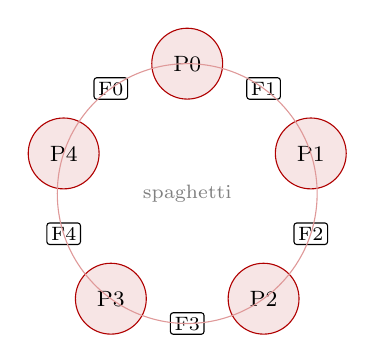
\begin{tikzpicture}[
                ph/.style={circle, draw=dp, fill=dp!10, font=\footnotesize, minimum size=9mm, inner sep=0pt},
                fk/.style={draw, fill=white, font=\scriptsize, rounded corners=1pt, inner sep=1.5pt}
            ]
                \foreach \i in {0,...,4} {
                    \pgfmathsetmacro{\a}{90-72*\i}
                    \pgfmathsetmacro{\b}{90-72*\i+36}
                    \node[ph] at (\a:1.65) {P\i};
                    \node[fk] at (\b:1.65) {F\i};
                }
                \draw[dp!40] (0,0) circle (1.65);
                \node[font=\scriptsize,gray] at (0,0) {spaghetti};
            \end{tikzpicture}

            \vspace{2pt}
            \scriptsize Philosopher $i$ needs forks $i$ and $(i+1) \bmod 5$.
        \end{column}
        \begin{column}{0.64\textwidth}
            \small
            \begin{itemize}
                \setlength\itemsep{2pt}
                \item Proposed by Dijkstra in 1965 \cite{downey}. A published
                    form is in \cite{dijkstra}.
                \item Five philosophers loop: think, get forks, eat, put forks.
                    Eating needs \textbf{two} forks.
                \item Required properties \cite{downey}:
                    \begin{itemize}
                        \item one holder per fork;
                        \item no deadlock and no starvation;
                        \item more than one philosopher can eat at once.
                    \end{itemize}
                \item \textbf{Deadlock:} each philosopher takes the first fork. All
                    five hold one fork and wait for the next. This is a
                    \textbf{circular wait}.
                \item Known fixes \cite{downey,tanenbaum}:
                    \begin{itemize}
                        \item allow only 4 at the table (\code{footman});
                        \item asymmetry: at least one philosopher takes forks in
                            the opposite order;
                        \item Tanenbaum: a state array plus one semaphore each.
                    \end{itemize}
            \end{itemize}
        \end{column}
    \end{columns}
\end{frame}

% ---------------------------------------------------------------- 5
\begin{frame}{Difference: Cigarette Smokers vs.\ Dining Philosophers}
    \footnotesize
    \renewcommand{\arraystretch}{1.15}
    \begin{tabular}{@{}>{\raggedright\bfseries}p{0.15\textwidth} >{\raggedright\arraybackslash}p{0.41\textwidth} >{\raggedright\arraybackslash}p{0.41\textwidth}@{}}
        \rowcolor{gray!15}
        & \textcolor{dp}{\textbf{Dining Philosophers}} & \textcolor{cs}{\textbf{Cigarette Smokers}} \\
        Origin & Dijkstra, 1965 \cite{downey}. Paper in 1971 \cite{dijkstra} & Patil, 1971 \cite{patil,downey} \\
        Threads & Five identical philosophers (peers) & One agent and three smokers with different roles \\
        Shared items & Five forks. Each fork sits between two neighbors and is put back after eating & Ingredients that the agent puts on the table. One smoker picks up both \\
        What a thread needs & Its two neighboring forks. Fixed by its seat & The two ingredients it lacks. Changes each round with the agent's random choice \\
        Who may proceed & Any philosopher whose two forks are free. Several can eat at once & Exactly one smoker per round. The agent waits for its signal \\
        Cause of deadlock & Circular wait: each philosopher holds one fork and waits for the next & Smokers take one needed item each, then wait. The wait cycle includes the agent \\
        Typical fix & Limit the seats, break the symmetry, or use a state array \cite{downey,tanenbaum} & Add helper threads (pushers) that track the table and wake the right smoker \cite{parnas,downey} \\
        Extra constraint & None beyond deadlock freedom, starvation freedom, and concurrency & Agent code stays unchanged \cite{downey} \\
        Models & Peers that compete for shared resources & An OS that allocates resource combinations to applications \cite{downey} \\
    \end{tabular}
\end{frame}

% ---------------------------------------------------------------- 6
\begin{frame}{What the differences mean}
    \begin{columns}[T]
        \begin{column}{0.49\textwidth}
            \small
            \textbf{Deadlock view.} Deadlock needs four conditions: mutual
            exclusion, hold and wait, no preemption, and circular wait
            \cite{coffman}.
            \vspace{3pt}
            \begin{itemize}
                \setlength\itemsep{3pt}
                \item \textcolor{dp}{\textbf{Philosophers:}} the circular wait is
                    among the peers. A fix removes the cycle (asymmetry) or
                    guarantees a free fork (4 seats).
                \item \textcolor{cs}{\textbf{Smokers:}} the problem is hold and
                    wait on a \emph{partial} set of ingredients. Pushers remove
                    it: a smoker is woken only when it can get both.
            \end{itemize}
        \end{column}
        \begin{column}{0.49\textwidth}
            \small
            \textbf{Three main differences}
            \begin{enumerate}
                \setlength\itemsep{3pt}
                \item \textbf{Peers vs.\ a driver.} Philosophers compete with
                    each other. In the smokers problem the agent decides who can
                    run.
                \item \textbf{Fixed vs.\ changing needs.} A philosopher always
                    needs the same two forks. A smoker's needs depend on the round.
                \item \textbf{Restrict vs.\ coordinate.} Philosopher fixes limit
                    or order the requests. The smokers fix add a thread that holds
                    the state and decides.
            \end{enumerate}
        \end{column}
    \end{columns}
    \vspace{4pt}
    \begin{block}{Takeaway}
        \small Taking resources one at a time can deadlock in both problems.
        Dining Philosophers asks how peers share fixed resources safely.
        Cigarette Smokers asks how to match changing resource sets to the one
        thread that can use them. Patil's restrictions decide whether
        semaphores are enough \cite{downey}.
    \end{block}
\end{frame}

% ---------------------------------------------------------------- references
\begin{frame}{References}
    \footnotesize
    \begin{thebibliography}{9}
        \bibitem{patil}
        S.~Patil, ``Limitations and Capabilities of Dijkstra's Semaphore
        Primitives for Coordination among Processes,'' Computation Structures
        Group Memo~57, Project MAC, MIT, Feb.\ 1971.
        \url{https://wiki.eecs.yorku.ca/course_archive/2014-15/W/6490A/_media/public:patil.pdf}

        \bibitem{parnas}
        D.~L. Parnas, ``On a solution to the cigarette smokers' problem
        (without conditional statements),'' \emph{Communications of the ACM},
        vol.~18, no.~3, pp.~181--183, Mar.\ 1975.
        \url{https://doi.org/10.1145/360680.360709}

        \bibitem{downey}
        A.~B. Downey, \emph{The Little Book of Semaphores}, 2nd ed., version
        2.2.2, Green Tea Press, 2016. Sections 4.5 and 4.6.
        \url{https://greenteapress.com/wp/semaphores/}

        \bibitem{dijkstra}
        E.~W. Dijkstra, ``Hierarchical ordering of sequential processes,''
        \emph{Acta Informatica}, vol.~1, no.~2, pp.~115--138, 1971.
        \url{https://doi.org/10.1007/BF00289519}

        \bibitem{tanenbaum}
        A.~S. Tanenbaum and H.~Bos, \emph{Modern Operating Systems}, 4th ed.,
        Pearson, 2015. Section 2.5.1, ``The Dining Philosophers Problem.''

        \bibitem{coffman}
        E.~G. Coffman, M.~J. Elphick, and A.~Shoshani, ``System deadlocks,''
        \emph{ACM Computing Surveys}, vol.~3, no.~2, pp.~67--78, Jun.\ 1971.
        \url{https://doi.org/10.1145/356586.356588}
    \end{thebibliography}
\end{frame}

\end{document}
